\chapter{Manejo de Gráficos.}

\section{Paquete {\bf graphicx}}

{\bf Ejemplo. Crecimiento Malthusiano}

El modelo de crecimiento de Malthus consiste en el problema de valores iniciales:

\begin{equation}
    \dot{x}(t)=\kappa x(t)
\end{equation}
con condición inicial $x(0)=X_0$.

 Tiene la solución 
\begin{equation}
    x(t)=X_0\mathrm{e}^{\kappa t}
\end{equation}

\begin{figure}[h!]
    \centering
    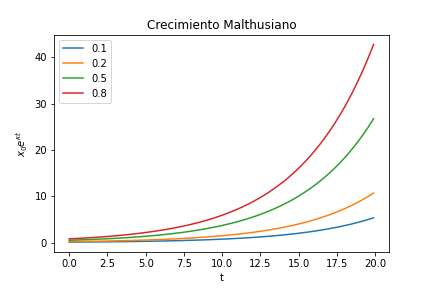
\includegraphics[scale=0.5]{malthus2.png}
    \caption{Gráfica para varias condiciones iniciales y $\kappa = 0.2$}
    \label{g2}
\end{figure}

\begin{figure}[h]
    \centering
    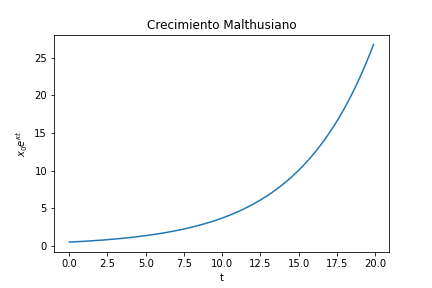
\includegraphics[scale=0.5]{malthus.png}
    \caption{Gráfica para $X_0=0.5$, $\kappa = 0.2$}
    \label{g1}
\end{figure}

 En la figura \ref{g1} podemos ver una solución para el crecimiento Malthusiano...

 \pgfplotsset{width=\textwidth,compat=1.9}

 \begin{figure}[h!]
     \centering
     \begin{tikzpicture}
         \begin{axis}[title={\bf Crecimiento Malthusiano},xlabel={\bf $t$},ylabel={\bf $X_0\rm{e}^{\kappa t}$},xmin=0,ymax=1.8]
             \addplot[color=blue]{0.5*exp(0.2*x)};
         \end{axis}
     \end{tikzpicture}
     \caption{Grafica Malthus pgfplots}
     \label{g3}
 \end{figure}

 \begin{figure}[h!]
    \centering
    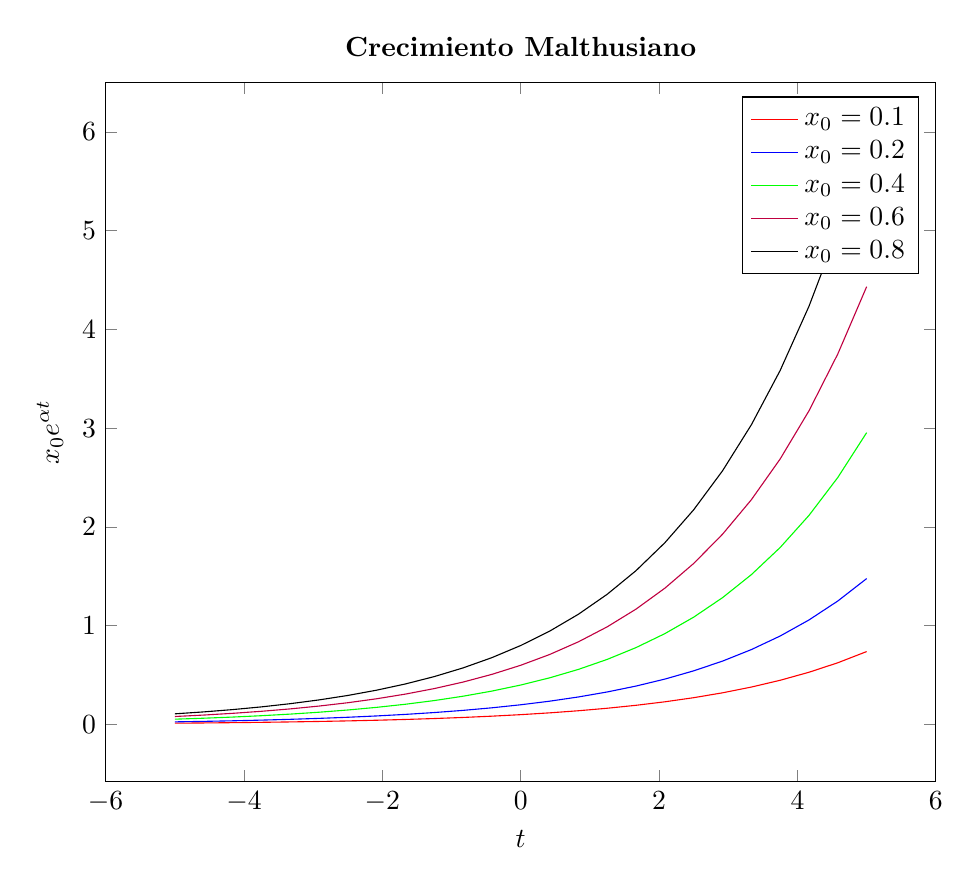
\begin{tikzpicture}
\begin{axis}[title={\bf Crecimiento Malthusiano},xlabel={\bf $t$},ylabel={\bf $x_0e^{\alpha t}$}]
\addplot[color=red]{0.1*exp(0.4*x)};\addlegendentry{$x_0=0.1$}
\addplot[color=blue]{0.2*exp(0.4*x)};\addlegendentry{$x_0=0.2$}
\addplot[color=green]{0.4*exp(0.4*x)};\addlegendentry{$x_0=0.4$}
\addplot[color=purple]{0.6*exp(0.4*x)};\addlegendentry{$x_0=0.6$}
\addplot[color=black]{0.8*exp(0.4*x)};\addlegendentry{$x_0=0.8$}
\end{axis}
\end{tikzpicture}
    \caption{Gráfica para varias condiciones iniciales y $\kappa = 0.4$}
    \label{g4}
\end{figure}